\documentclass[CJK]{beamer}
\usepackage{CJKutf8}
\usepackage{graphicx}
%\usetheme{Copenhagen}
\usetheme{Boadilla}
\setbeamercovered{transparent}

\begin{document}
\begin{CJK*}{UTF8}{gbsn}

\title{计算机编程基础与实践}
\subtitle{---课程大实验概述}
\author{夏永锋}
\institute[SJTU]
{上海交通大学\ 软件学院\\嵌入式实验室}
\date{\today}

\begin{frame}
	\titlepage
\end{frame}

\begin{frame}{Web数据库架构的工作原理}
\begin{center}
	\includegraphics[width=9cm]{webDatabase.png}
\end{center}
{\small
\begin{block}{}
\begin{enumerate}
	\item 一个用户的浏览器发出一个HTTP请求,请求特定的Web页面;
	\item Web服务器接收到对某个php页面的请求后,检索该文件,并将其传递给PHP引擎进行处理;
	\item PHP引擎开始解析脚本。脚本主要包括了连接到数据库和执行查询的命令。PHP启动了对MySQL服务器的连接并向该服务器发送适当的查询;
	\item MySQL服务器接收到数据库查询的请求,开始处理这个查询,并将查询结果返回给PHP引擎;
	\item PHP引擎完成了脚本的运行后(其中包括以HTML格式表示处理后的查询结果),然后将该HTML返回给Web服务器;
	\item Web服务器再将HTML返回给客户端浏览器,用户就可以看到结果了。
\end{enumerate}
\end{block}
}
\end{frame}
\begin{frame}{续}
\begin{center}
	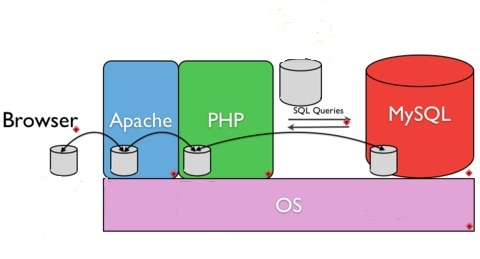
\includegraphics[width=10cm]{AMP.jpg}
\end{center}
\end{frame}
\begin{frame}{续}
\begin{center}
	\includegraphics[width=12cm]{detail.png}
\end{center}
\end{frame}
\begin{frame}{续}
\begin{block}{}
通常,Web服务器软件,PHP引擎和数据库服务器都在同一台机器上运行。但是,有时会出于保密,提高性能以及负载平衡的等考虑,而将数据库服务器运行在另外一条机器上。
\end{block}
\end{frame}
\begin{frame}{实验内容概述}
\begin{block}{}
{\bf	实现一个Browser/Server模式的简单数据库应用 --- 简单通讯录}
\end{block}
\begin{block}{}
{\bf 实验环境:}Linux, PHP, MySQL\\
{\bf 要求:}联系人的添加,删除,修改
\end{block}
因此,主要包括如下三个方面的工作:
\begin{block}{}
	\begin{itemize}
		\item 如何存储?---数据库的设计
		\item 如果存取?---通过PHP+SQL访问数据库
		\item 交互界面---使用HTML(HyperText Markup Language)
	\end{itemize}
\end{block}
\end{frame}

\begin{frame}
	\begin{center}
	{\LARGE THANK YOU !}
	\end{center}
	\begin{block}{}
	\begin{center}
	{\small Proud to use \LaTeX\ and Beamer.}
	\end{center}
	\end{block}
\end{frame}

\end{CJK*}
\end{document}
